\documentclass[10pt]{beamer}
% \usetheme{Boadilla}
  \usetheme{default}


% acronyms for text or math mode
\newcommand {\ccast} {\mbox{\small\textsc{ccast}}}
\newcommand {\kcarta} {\mbox{k\small{CARTA}}}

\newcommand {\cris} {\mbox{\small CrIS}}
\newcommand {\airs} {\mbox{\small AIRS}}
\newcommand {\iasi} {\mbox{\small IASI}}
\newcommand {\idps} {\mbox{\small IDPS}}
\newcommand {\nasa} {\mbox{\small NASA}}
\newcommand {\noaa} {\mbox{\small NOAA}}
\newcommand {\nstar} {\mbox{\small STAR}}
\newcommand {\umbc} {\mbox{\small UMBC}}
\newcommand {\uw}   {\mbox{\small UW}}

\newcommand {\fft}  {\mbox{\small FFT}}
\newcommand {\ifft} {\mbox{\small IFFT}}
\newcommand {\fir}  {\mbox{\small FIR}}
\newcommand {\fov}  {\mbox{\small FOV}}
\newcommand {\for}  {\mbox{\small FOR}}
\newcommand {\ict}  {\mbox{\small ICT}}
\newcommand {\ils}  {\mbox{\small ILS}}
\newcommand {\igm}  {\mbox{\small IGM}}
\newcommand {\opd}  {\mbox{\small OPD}}
\newcommand {\rms}  {\mbox{\small RMS}}
\newcommand {\zpd}  {\mbox{\small ZPD}}
\newcommand {\ppm}  {\mbox{\small PPM}}
\newcommand {\srf}  {\mbox{\small SRF}}
\newcommand {\sdr}  {\mbox{\small SDR}}
\newcommand {\FWHM} {\mbox{\small FWHM}}
\newcommand {\fwhm} {\mbox{\small\textsc{fwhm}}}

\newcommand {\ES} {\mbox{\small ES}}
\newcommand {\SP} {\mbox{\small SP}}
\newcommand {\IT} {\mbox{\small IT}}
\newcommand {\SA} {\mbox{\small SA}}

\newcommand {\ET} {\mbox{\small ET}}
\newcommand {\FT} {\mbox{\small FT}}

\newcommand {\wn} {\mbox{cm$^{-1}$}}
\newcommand {\cm} {\mbox{cm}}

% abbreviations, mainly for math mode
\newcommand {\real} {\mbox{real}}
\newcommand {\imag} {\mbox{imag}}
\newcommand {\atan} {\mbox{atan}}
\newcommand {\obs}  {\mbox{obs}}
\newcommand {\calc} {\mbox{calc}}
\newcommand {\sinc} {\mbox{sinc}}
\newcommand {\psinc} {\mbox{psinc}}
\newcommand {\std} {\mbox{std}}

% symbols, for math mode only
\newcommand {\lmax} {L_{\mbox{\tiny max}}}
\newcommand {\vmax} {V_{\mbox{\tiny max}}}

\newcommand {\tauobs} {\tau_{\mbox{\tiny obs}}}
\newcommand {\taucal} {\tau_{\mbox{\tiny calc}}}
\newcommand {\Vdc}  {V_{\mbox{\tiny DC}}}

\newcommand {\rIT} {r_{\mbox{\tiny\textsc{ict}}}}
\newcommand {\rES} {r_{\mbox{\tiny\textsc{es}}}}
\newcommand {\robs} {r_{\mbox{\tiny obs}}}

\newcommand {\rITobs} {r_{\mbox{\tiny\textsc{ict}}}^{\mbox{\tiny obs}}}
\newcommand {\rITcal} {r_{\mbox{\tiny\textsc{ict}}}^{\mbox{\tiny cal}}}

\newcommand {\rESuser} {r_{\mbox{\tiny\textsc{es}}}^{\mbox{\tiny user}}}
\newcommand {\rITuser} {r_{\mbox{\tiny\textsc{ict}}}^{\mbox{\tiny user}}}
\newcommand {\rITsensor} {r_{\mbox{\tiny\textsc{ict}}}^{\mbox{\tiny sensor}}}
\newcommand {\rITfov} {r_{\mbox{\tiny\textsc{ict}}}^{\mbox{\tiny fov}}}

\newcommand {\fcos} {f_{\mbox{\tiny cos}}}
\newcommand {\fatbd} {f_{\mbox{\tiny\textsc{atbd}}}}

\newcommand {\ITmean} {\langle\mbox{\small IT}\rangle}
\newcommand {\SPmean} {\langle\mbox{\small SP}\rangle}

\newcommand {\Ttc} {t^{\mbox{\tiny\textsc{tc}}}}
\newcommand {\Tac} {t^{\mbox{\tiny\textsc{ac}}}}
\newcommand {\rtc} {r_{\mbox{\tiny\textsc{tc}}}}
\newcommand {\rta} {r_{\mbox{\tiny\textsc{ta}}}}



\title{A first look at the 7-8 Jan 2020\\
  CrIS TVAC PFL gas cell tests}
\author{H.~E.~Motteler, L.~L.~Strow, \\
  S.~DeSouza-Machado, \\
  S.~Buczkowski
}
\institute{
  UMBC Atmospheric Spectroscopy Lab \\
  Joint Center for Earth Systems Technology \\
}
\date{\today}
\begin{document}

%----------- slide --------------------------------------------------%
\begin{frame}[plain]
\titlepage
\end{frame}
%----------- slide --------------------------------------------------%
\begin{frame}
\frametitle{Introduction}
\begin{itemize}

  \item We do a preliminary analysis of the PFL Plateau 20 CH$_4$,
    CO$_2$, and CO gas cell tests, and compare these with calculated
    reference truth.

  \item These initial results look fairly good, but we have taken
    some shortcuts, including using less than optimal test interval
    subsets and (for CO$_2$ and CO) older transmittance calcs that do
    not quite match the current cell parameters.
 
  \item Working from our metrology laser residuals we show focal
    plane fits for all three CrIS bands.

  \item We have included examples of monitoring the test logs
    (the CSS, CMD, and TCR files), in the form of plots of HTBB
    temperature, gas cell temperature and gas cell pressure over
    time.

  \item The J2 tests appear to have been done at the older
    866/1052/799 point resolutions.  This is not a problem for us,
    but was unexpected.
    
\end{itemize}
\end{frame}
%----------- slide --------------------------------------------------%
\begin{frame}
\frametitle{Methods}
\begin{itemize}

  \item For each gas we partition the data stream into four test
    legs, \\ FT1, FT2, ET1, and ET2 (cell full, HTBB temperature T1,
    etc.)

  \item For test each leg, we take the mean of the associated count
    spectra, calculate the transmittance as $(FT2 - FT1) / (ET2 -
    ET1)$, apply the SA correction, and interpolate to a finer grid
    for residual analysis.
    
  \item This is similar in some ways to the ``ratio first''
    calibration algorithm used as an option in UMBC CCAST
    processing, but note that we do not do a full radiance
    calibration, or any nonlinearity correction, for the analysis
    here.

  \item Measured and calculated transmittances are compared by
    fitting obs to calcs and then examining fitting weights and
    residuals.

  \item This approach, with fitting adjustments, is acceptable for
    our application because our main task is spectral calibration
    and our fitting methods are robust in the face of radiometric
    uncertainty.

\end{itemize}
\end{frame}
%----------- slide --------------------------------------------------%
\begin{frame}
\frametitle{7-8 Jan 2020 TVAC PFL Plateau 20}
\begin{columns}[t]
\begin{column}{0.5\textwidth}
  \begin{centering}
  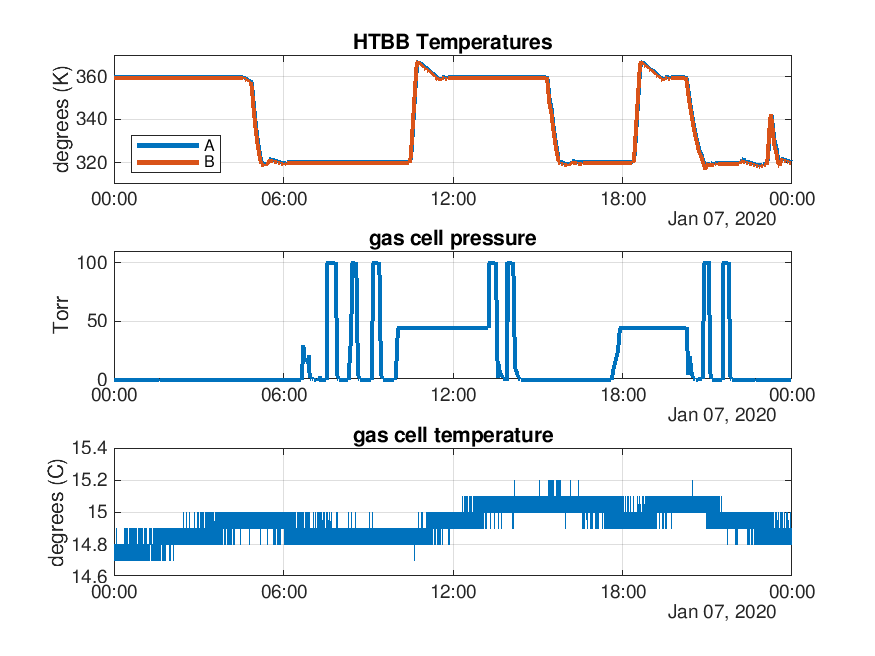
\includegraphics[width=\textwidth]{figures/css_summary_07_jan.png}
  \end{centering}\vspace{3mm}

\end{column}
\begin{column}{0.5\textwidth}  
  \begin{centering}
  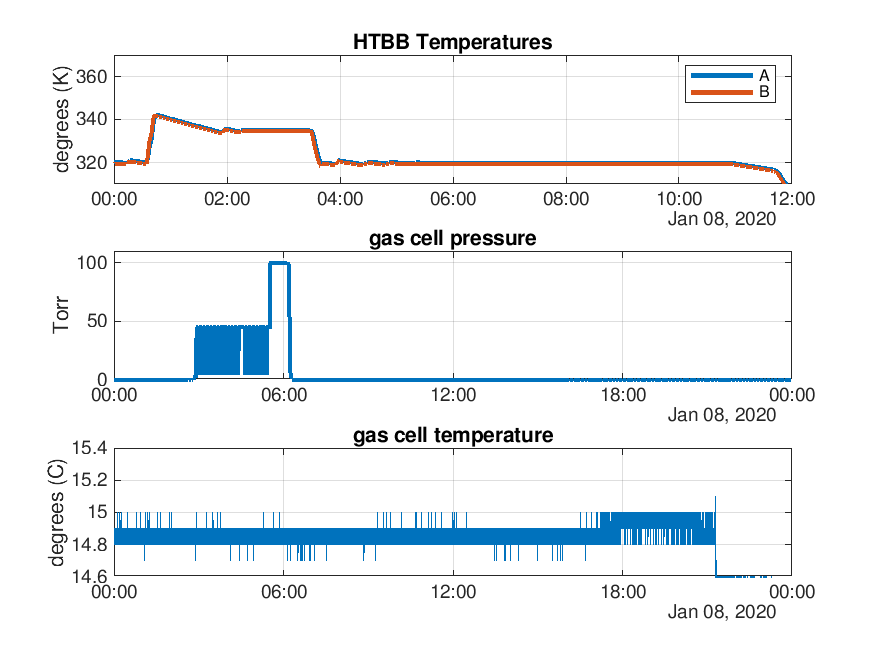
\includegraphics[width=\textwidth]{figures/css_summary_08_jan.png}
  \end{centering}\vspace{3mm}

\end{column}
\end{columns}

HTBB temperatures, gas cell pressure and gas cell temperature from
the CCS files, for 7-8 Jan 2020.  This data is used along with a
scan of the CMD and SQL files to find the test stages.

\end{frame}
%----------- slide --------------------------------------------------%
\begin{frame}
\frametitle{7 Jan MW CH4 cell empty test legs}
\begin{columns}[t]
\begin{column}{0.5\textwidth}
  \begin{centering}
  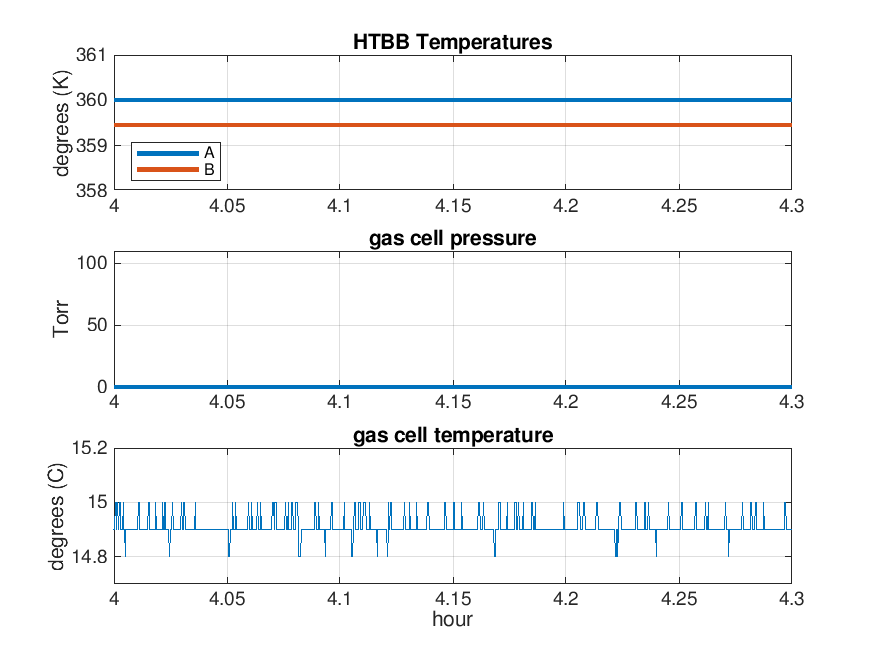
\includegraphics[width=\textwidth]{figures/MW_high_empty_gas_unknown.png}
  \end{centering}\vspace{3mm}

 ``empty high'' leg of the the 7 Jan transmittance test, PFL Plateau
  20.  The x-axis here is hour of the day for 7 Jan.  This data
  looks good.

\end{column}
\begin{column}{0.5\textwidth}  
  \begin{centering}
  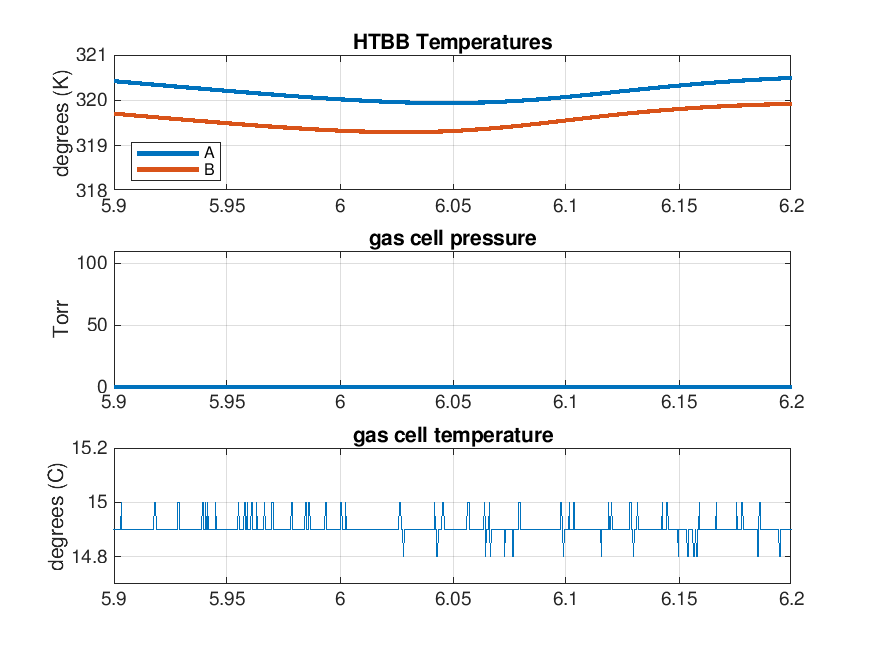
\includegraphics[width=\textwidth]{figures/MW_low_empty_gas_unknown.png}
  \end{centering}\vspace{3mm}

 ``empty low'' leg of the the 7 Jan transmittance test.  The x-axis
  is again hour of the day.  We see some HTBB drift.

\end{column}
\end{columns}
\end{frame}
%----------- slide --------------------------------------------------%
\begin{frame}
\frametitle{7 Jan MW CH4 cell full test legs}
\begin{columns}[t]
\begin{column}{0.5\textwidth}
  \begin{centering}
  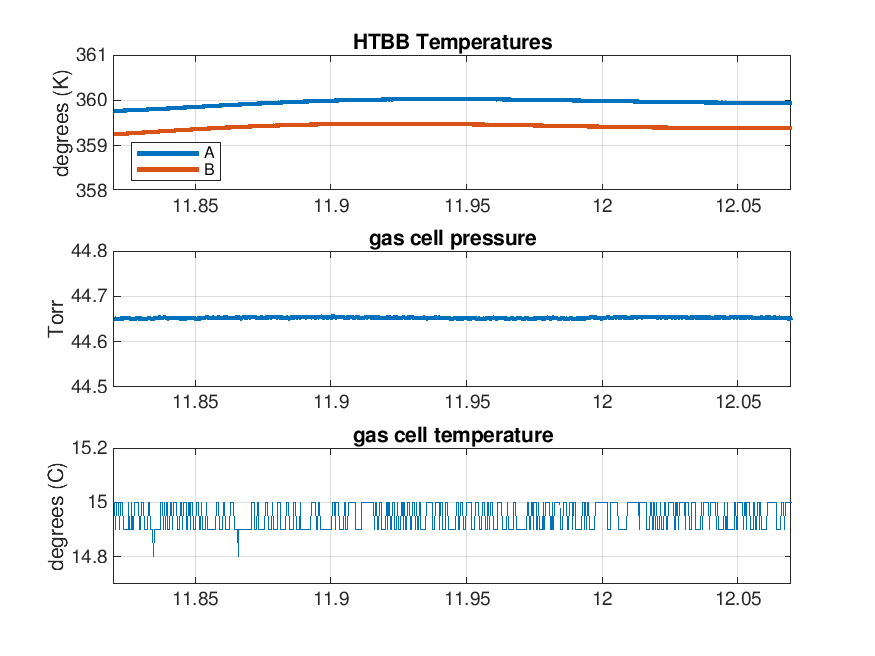
\includegraphics[width=\textwidth]{figures/MW_high_full_gas_unknown.png}
  \end{centering}\vspace{3mm}

 ``full high'' leg of the the 7 Jan \\ CH4 transmittance test.  The
  x-axis is hour of the day.  As in the empty low leg we see some
  HTBB drift.

\end{column}
\begin{column}{0.5\textwidth}  
  \begin{centering}
  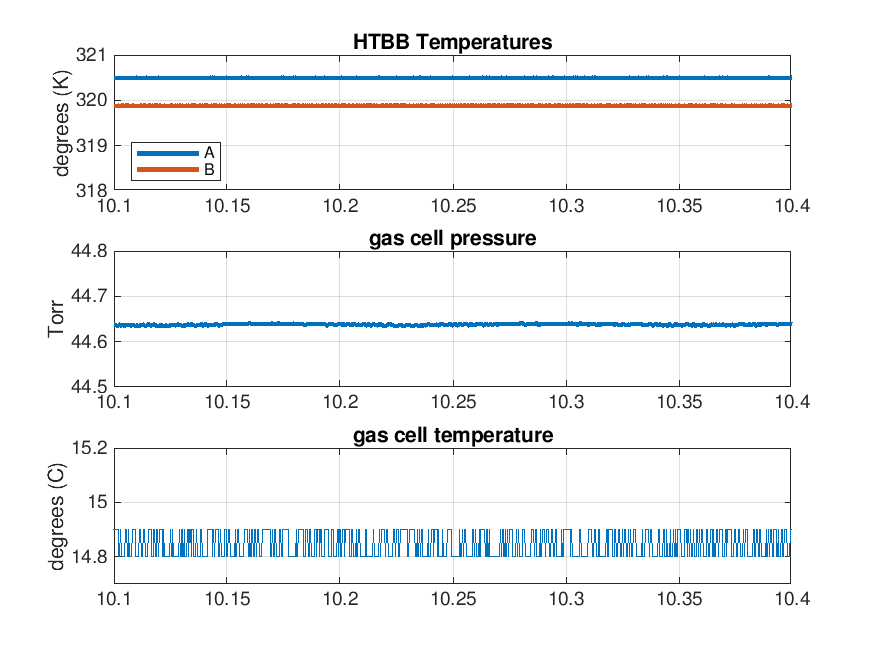
\includegraphics[width=\textwidth]{figures/MW_low_full_gas_unknown.png}
  \end{centering}\vspace{3mm}

 ``full low'' leg of the the 7 Jan CH4 transmittance test.  This
  looks good.

\end{column}
\end{columns}
\end{frame}
%----------- slide --------------------------------------------------%
\begin{frame}
\frametitle{CH4 MW test parameters}

\begin{itemize}
  \item PFL Plateau 20, 7-8 Jan 2019
  \item side 1, sweep direction 0
  \item fitting interval 1220 to 1380 $\wn$
  \item metrology laser 773.0764 nm, from neon 703.4476 nm
  \item ATBD default focal plane
  \item SA correction from ILS with periodic sinc at the sensor grid
% \item obs/test leg: ET1 533, ET2 364, FT1 344, FT2 364
  \item HTBB nominal T1 360 K, T2 320 K
  \item gas cell pressure 44.64 torr
  \item gas cell temperature 14.85 C
  \item gas cell length 12.59 cm
\end{itemize}

\end{frame}
%----------- slide --------------------------------------------------%
\begin{frame}
\frametitle{CH4 data before fitting}
\begin{columns}[t]
\begin{column}{0.5\textwidth}  
  \begin{centering}
  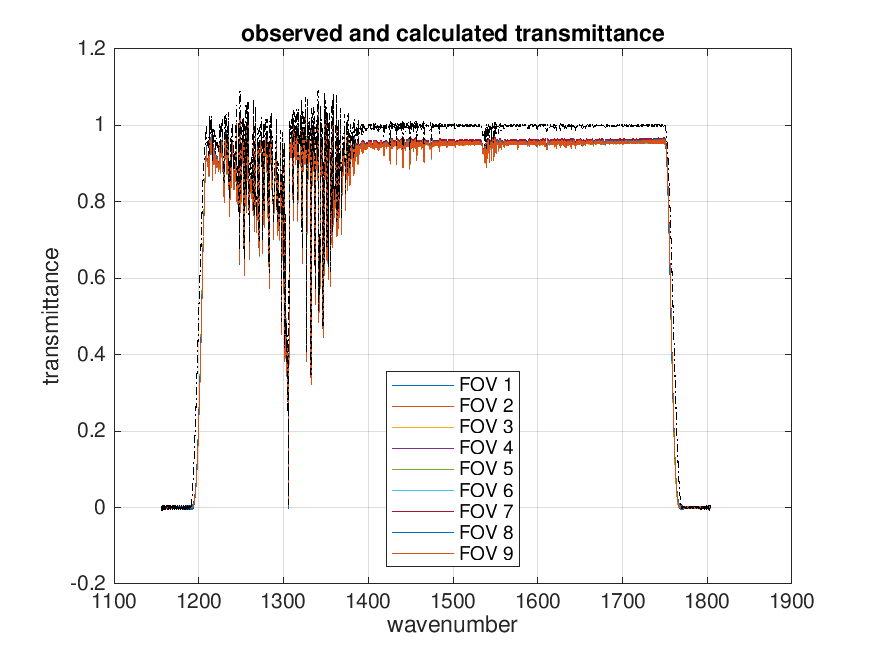
\includegraphics[width=\textwidth]{figures/spec_test2_CH4_all.png}
  \end{centering}\vspace{3mm}

Observed and calculated transmittance after the SA correction but
before fitting.  We see a significant bias in the obs, possibly due
to problems with the HTBB or gas cell stability.  More careful
subsetting of the test data would probably fix this.

\end{column}

\begin{column}{0.5\textwidth}
  \begin{centering}
  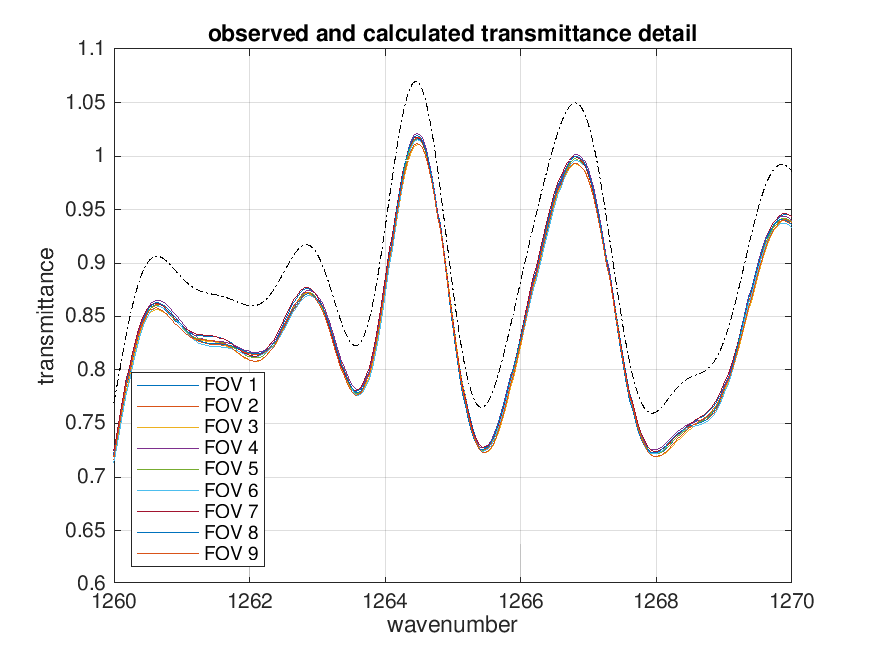
\includegraphics[width=\textwidth]{figures/spec_test2_CH4_zoom.png}
  \end{centering}\vspace{3mm}

A detail from the previous plot. Despite the bias, the FOV to FOV
consistency of the observed data is relatively good.

\end{column}
\end{columns}
\end{frame}
%----------- slide --------------------------------------------------%
\begin{frame}
\frametitle{CH4 fitting overview}
\begin{columns}[t]
\begin{column}{0.5\textwidth}  
  \begin{centering}
  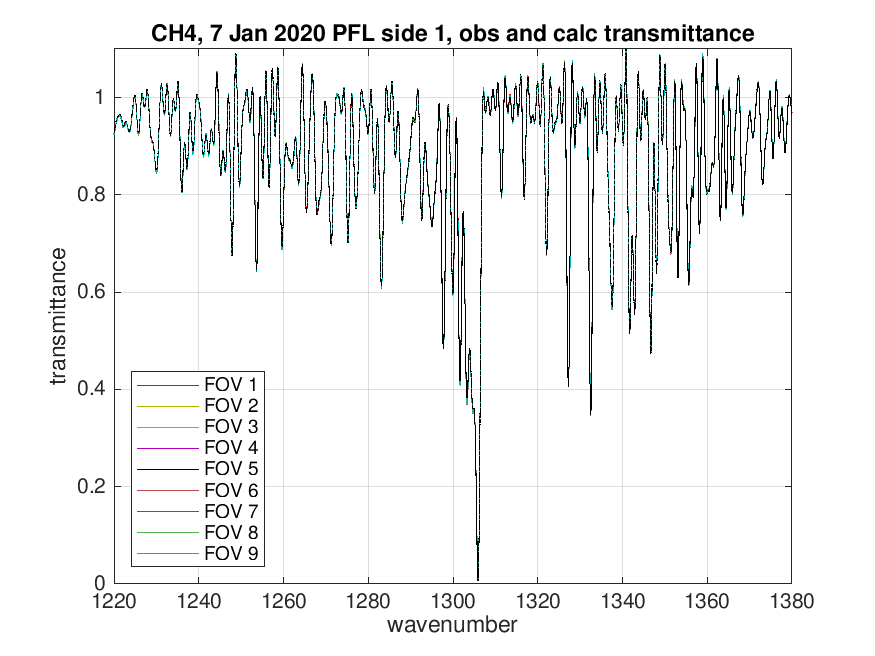
\includegraphics[width=\textwidth]{figures/CH4_obs_and_calc.png}
  \end{centering}\vspace{3mm}

Observed and calculated transmittance for all FOVs, over the fitting
interval.  At this level of detail we see all values are very close.

\end{column}

\begin{column}{0.5\textwidth}
  \begin{centering}
  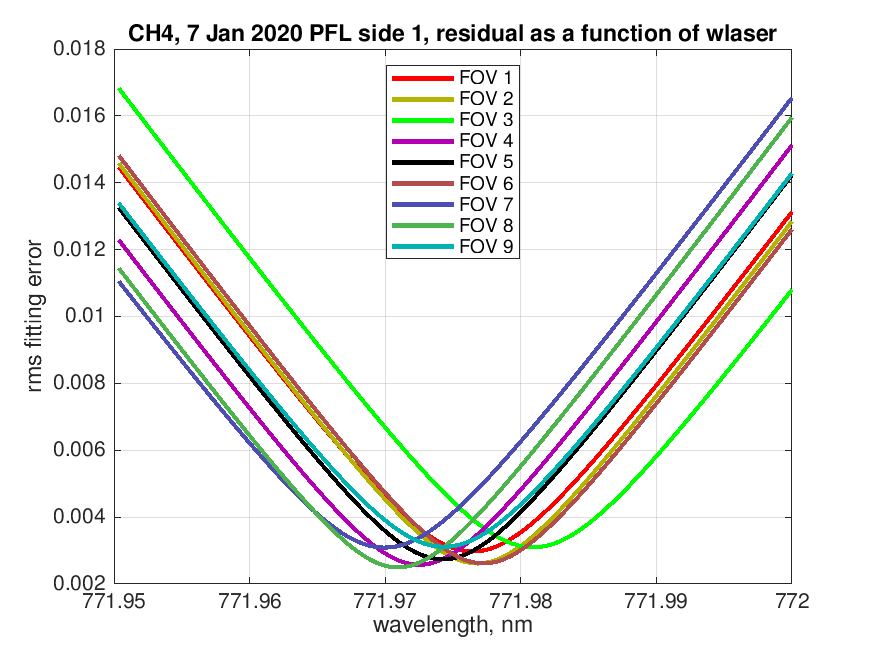
\includegraphics[width=\textwidth]{figures/CH4_wlaser_fit.png}
  \end{centering}\vspace{3mm}

Residuals $\rms(a\cdot\tauobs + b - \taucal)$ over the fitting
interval as a function of metrology laser wavelength, for each FOV.

\end{column}
\end{columns}
\end{frame}
%----------- slide --------------------------------------------------%
\begin{frame}
\frametitle{CH4 obs minus calc breakouts}
\begin{columns}[t]
\begin{column}{0.5\textwidth}
  \begin{centering}
  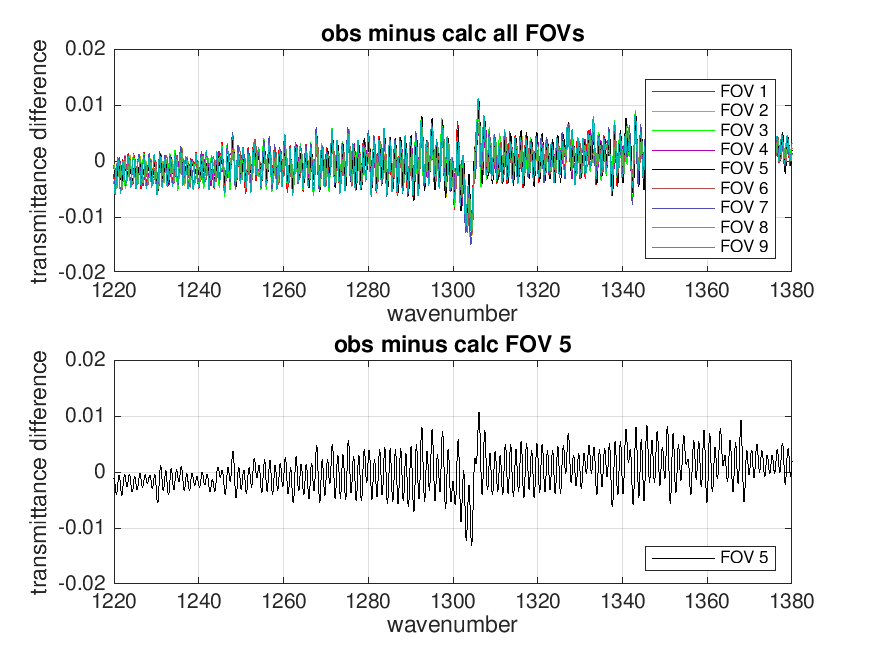
\includegraphics[width=\textwidth]{figures/CH4_breakout_1.png}
  \end{centering}\vspace{3mm}

Observed minus calculated transmittance for all FOVs and for FOV~5
alone, over the fitting interval.

\end{column}
\begin{column}{0.5\textwidth}  
  \begin{centering}
  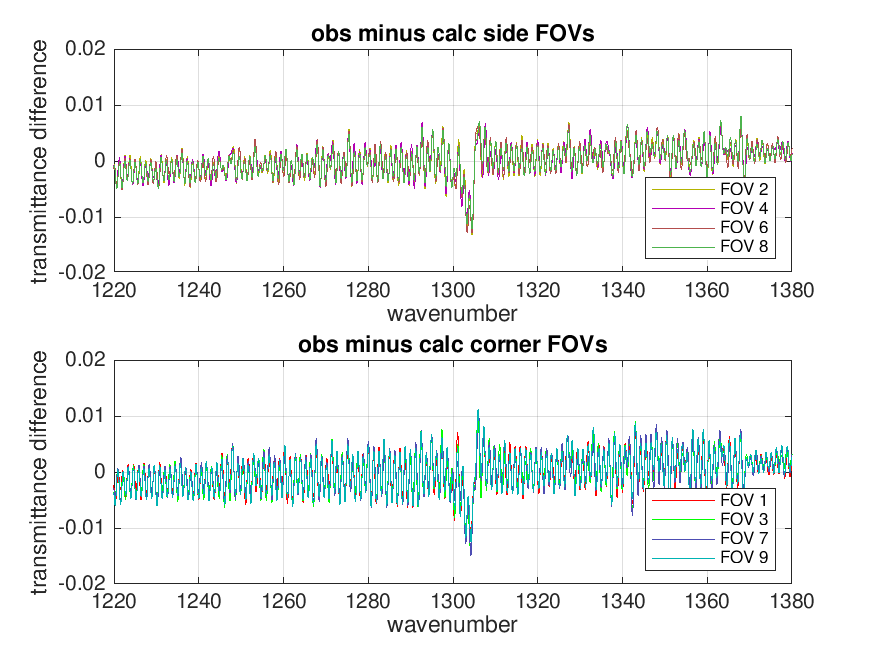
\includegraphics[width=\textwidth]{figures/CH4_breakout_2.png}
  \end{centering}\vspace{3mm}

Observed minus calculated transmittance for side and corner FOVs,
over the fitting interval.

\end{column}
\end{columns}
\end{frame}
%----------- slide --------------------------------------------------%
\begin{frame}[fragile]
\frametitle{CH4 tabulated residuals}

  metrology laser absolute residuals, ppm
\begin{semiverbatim}\scriptsize
     -0.65     2.59     7.77         7   4   1
      0.65     5.18     8.42         8   5   2
      5.18     9.07    13.60         9   6   3
\end{semiverbatim}

  metrology laser relative residuals, ppm
\begin{semiverbatim}\scriptsize
     -5.83    -2.59     2.59         7   4   1
     -4.53     0.00     3.24         8   5   2
      0.00     3.89     8.42         9   6   3
\end{semiverbatim}

     regression fitting weights and residuals
\begin{semiverbatim}\scriptsize
 FOV   "a"       "b"     dmin     wmin      wfov
  1   1.035    0.0135   0.0030     7.77   771.9764 
  2   1.040    0.0115   0.0026     8.42   771.9769 
  3   1.041    0.0130   0.0031    13.60   771.9809 
  4   1.036    0.0115   0.0026     2.59   771.9724 
  5   1.038    0.0127   0.0027     5.18   771.9744 
  6   1.043    0.0107   0.0026     9.07   771.9774 
  7   1.035    0.0119   0.0031    -0.65   771.9699 
  8   1.038    0.0128   0.0025     0.65   771.9709 
  9   1.041    0.0118   0.0031     5.18   771.9744 
\end{semiverbatim}

\end{frame}
%----------- slide --------------------------------------------------%
\begin{frame}
\frametitle{CO2 LW test parameters}

\begin{itemize}
  \item PFL Plateau 20, 7-8 Jan 2019
  \item side 1, sweep direction 0
  \item fitting interval 672 to 712 $\wn$
  \item metrology laser 771.97035 nm, from neon 703.44765 nm
  \item ATBD default focal plane
  \item SA correction from ILS with periodic sinc at the sensor grid
% \item 364 x 9 obs/test leg
  \item HTBB nominal T1 360 K, T2 320 K
  \item gas cell pressure 45.05 torr
  \item gas cell temperature 15.0 C
  \item gas cell length 12.59 cm
\end{itemize}

\end{frame}
%----------- slide --------------------------------------------------%
\begin{frame}
\frametitle{CO2 data before fitting}
\begin{columns}[t]
\begin{column}{0.5\textwidth}  
  \begin{centering}
  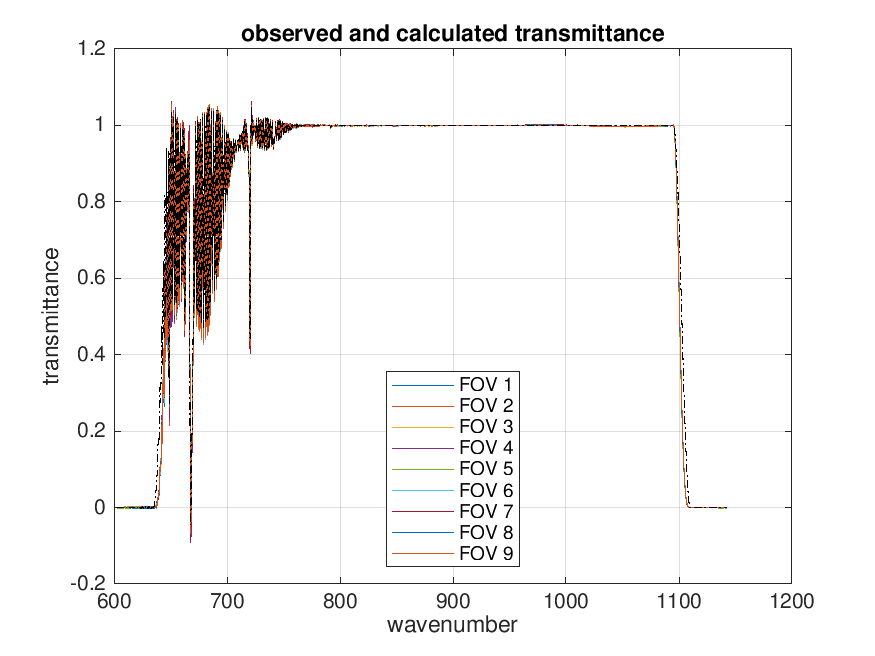
\includegraphics[width=\textwidth]{figures/spec_test2_CO2_all.png}
  \end{centering}\vspace{3mm}

Observed and calculated transmittance after the SA correction but
before any fitting.  This looks fairy good, despite some mismatch
in the calculated and actual gas cell parameters.

\end{column}

\begin{column}{0.5\textwidth}
  \begin{centering}
  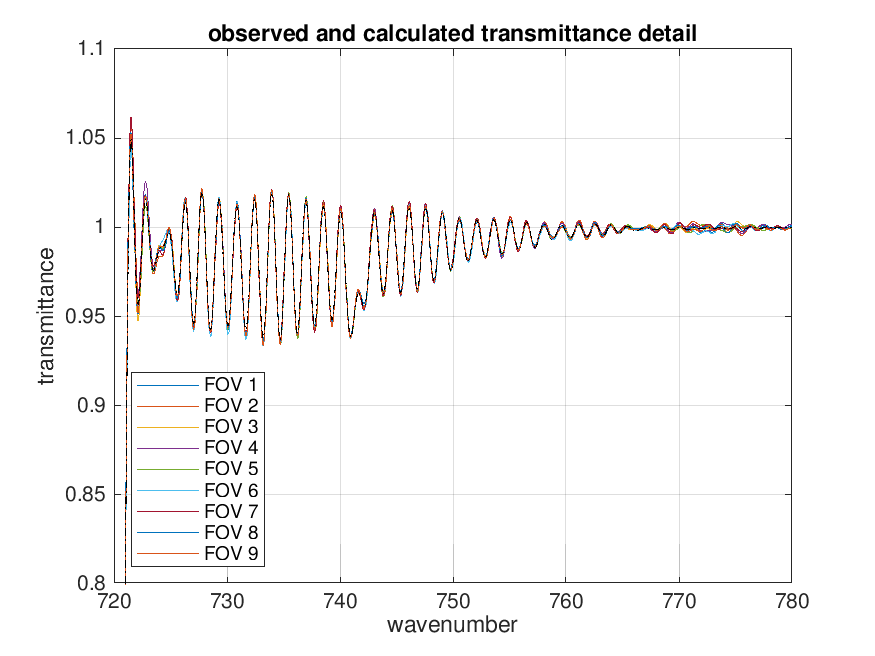
\includegraphics[width=\textwidth]{figures/spec_test2_CO2_zoom.png}
  \end{centering}\vspace{3mm}

A detail from the previous plot. \\ The FOV to FOV consistency and
agreement with calculated transmittance is fairly good.

\end{column}
\end{columns}
\end{frame}
%----------- slide --------------------------------------------------%
\begin{frame}
\frametitle{CO2 fitting overview}
\begin{columns}[t]
\begin{column}{0.5\textwidth}  
  \begin{centering}
  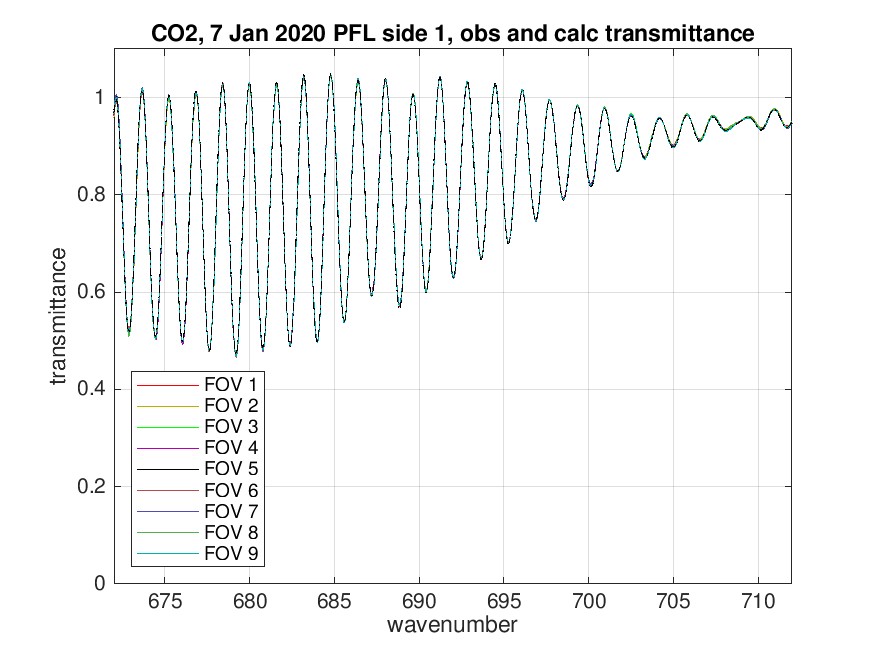
\includegraphics[width=\textwidth]{figures/CO2_obs_and_calc.png}
  \end{centering}\vspace{3mm}

Observed and calculated transmittance for all FOVs, over the fitting
interval.  At this level of detail we see all values are very close.

\end{column}

\begin{column}{0.5\textwidth}
  \begin{centering}
  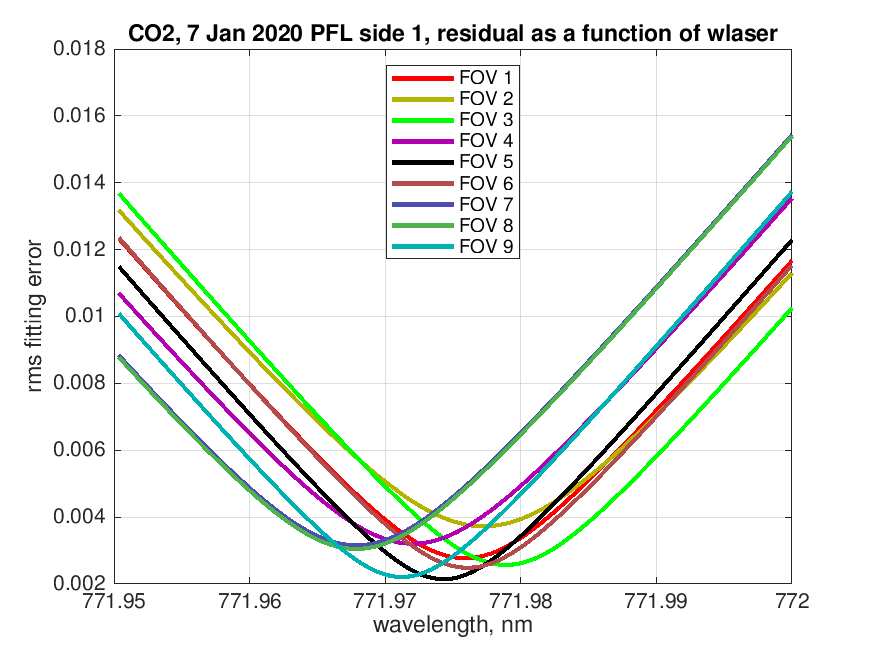
\includegraphics[width=\textwidth]{figures/CO2_wlaser_fit.png}
  \end{centering}\vspace{3mm}

Residuals $\rms(a\cdot\tauobs + b - \taucal)$ over the fitting
interval as a function of metrology laser wavelength, for each FOV.

\end{column}
\end{columns}
\end{frame}
%----------- slide --------------------------------------------------%
\begin{frame}
\frametitle{CO2 obs minus calc breakouts}
\begin{columns}[t]
\begin{column}{0.5\textwidth}
  \begin{centering}
  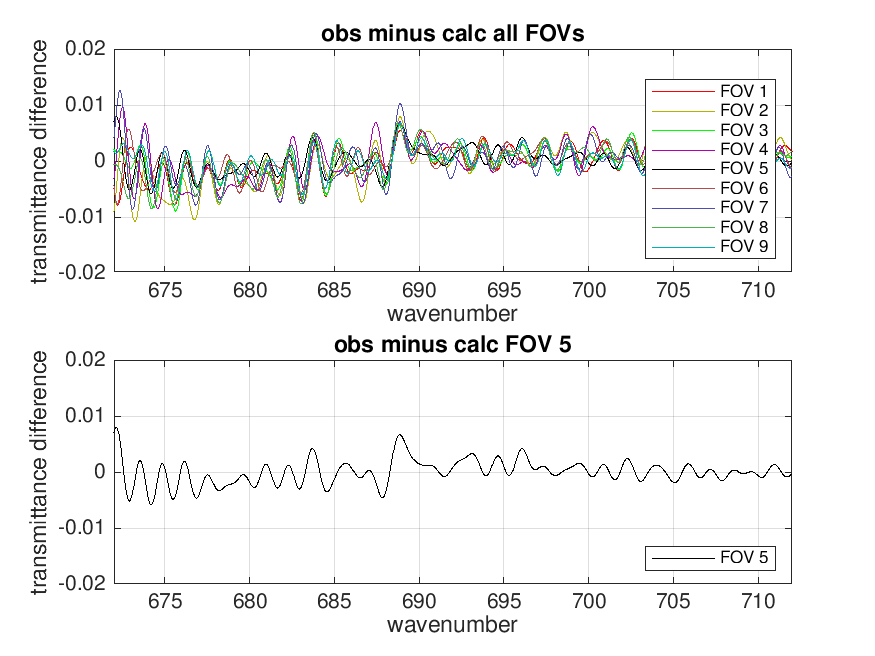
\includegraphics[width=\textwidth]{figures/CO2_breakout_1.png}
  \end{centering}\vspace{3mm}

Observed minus calculated transmittance for all FOVs and for FOV~5
alone, over the fitting interval.

\end{column}
\begin{column}{0.5\textwidth}  
  \begin{centering}
  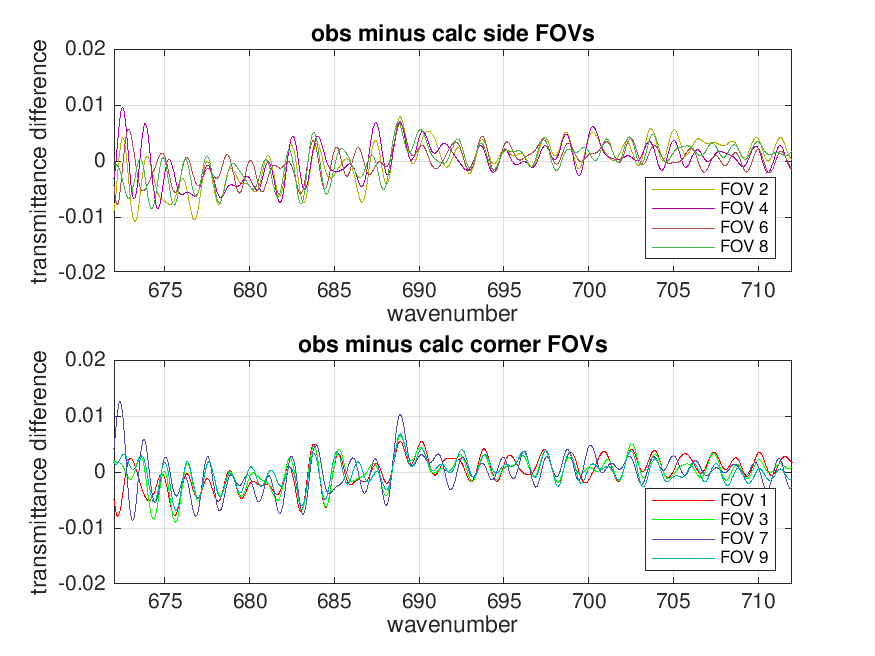
\includegraphics[width=\textwidth]{figures/CO2_breakout_2.png}
  \end{centering}\vspace{3mm}

Observed minus calculated transmittance for side and corner FOVs,
over the fitting interval.

\end{column}
\end{columns}
\end{frame}
%----------- slide --------------------------------------------------%
\begin{frame}[fragile]
\frametitle{CO2 tabulated residuals}

  metrology laser absolute residuals, ppm
\begin{semiverbatim}\scriptsize
     -3.24     1.94     7.12         7   4   1
     -3.24     5.18     9.07         8   5   2
      1.30     7.12    11.01         9   6   3
\end{semiverbatim}

  metrology laser relative residuals, ppm
\begin{semiverbatim}\scriptsize
     -8.42    -3.24     1.94         7   4   1
     -8.42     0.00     3.89         8   5   2
     -3.89     1.94     5.83         9   6   3
 \end{semiverbatim}

     regression fitting weights and residuals
\begin{semiverbatim}\scriptsize
 FOV   "a"       "b"     dmin     wmin      wfov
  1   0.937    0.0626   0.0028     7.12   771.9759 
  2   0.946    0.0552   0.0037     9.07   771.9774 
  3   0.930    0.0687   0.0026    11.01   771.9789 
  4   0.936    0.0622   0.0032     1.94   771.9719 
  5   0.926    0.0722   0.0021     5.18   771.9744 
  6   0.930    0.0689   0.0025     7.12   771.9759 
  7   0.935    0.0625   0.0032    -3.24   771.9679 
  8   0.944    0.0564   0.0030    -3.24   771.9679 
  9   0.930    0.0679   0.0022     1.30   771.9714 
\end{semiverbatim}

\end{frame}
%----------- slide --------------------------------------------------%
\begin{frame}
\frametitle{CO SW test parameters}

\begin{itemize}
  \item PFL Plateau 20, 8 Jan 2019
  \item side 1, sweep direction 0
  \item fitting interval 2160 to 2240 $\wn$
  \item metrology laser 771.97035 nm, from neon 703.44765 nm
  \item ATBD default focal plane
  \item SA correction from ILS with periodic sinc at the sensor grid
% \item 364 x 9 obs/test leg (check this)
  \item HTBB nominal T1 335 K, T2 320 K
  \item gas cell pressure 45.9 torr
  \item gas cell temperature 14.85 C
  \item gas cell length 12.59 cm
\end{itemize}

\end{frame}
%----------- slide --------------------------------------------------%
\begin{frame}
\frametitle{CO data before fitting}
\begin{columns}[t]
\begin{column}{0.5\textwidth}  
  \begin{centering}
  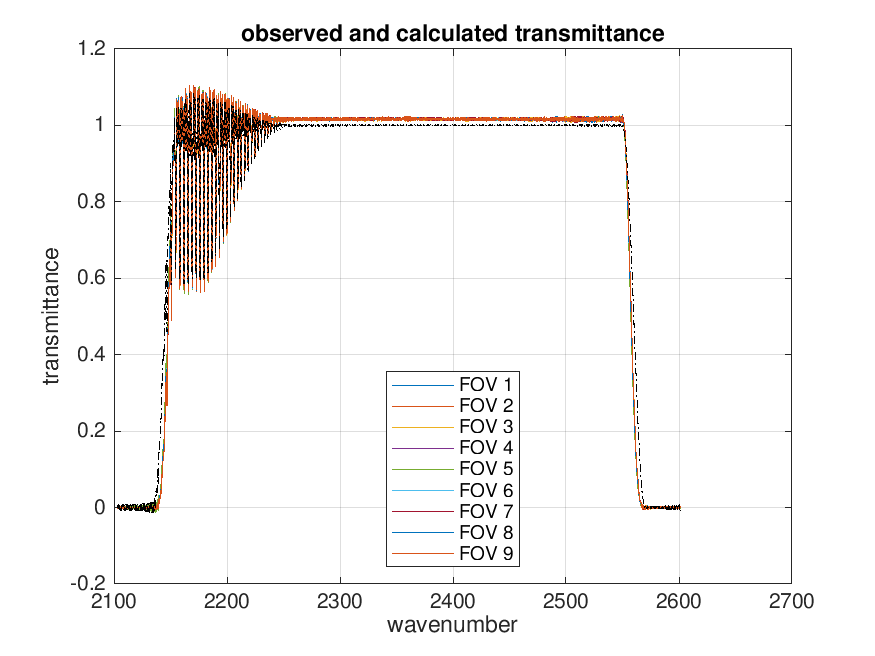
\includegraphics[width=\textwidth]{figures/spec_test2_CO_all.png}
  \end{centering}\vspace{3mm}

Observed and calculated transmittance after the SA correction but
before fitting.  We see some bias in the obs, though not as much as
for CH4.  As in that case, more careful subsetting would probably
improve this.

\end{column}

\begin{column}{0.5\textwidth}
  \begin{centering}
  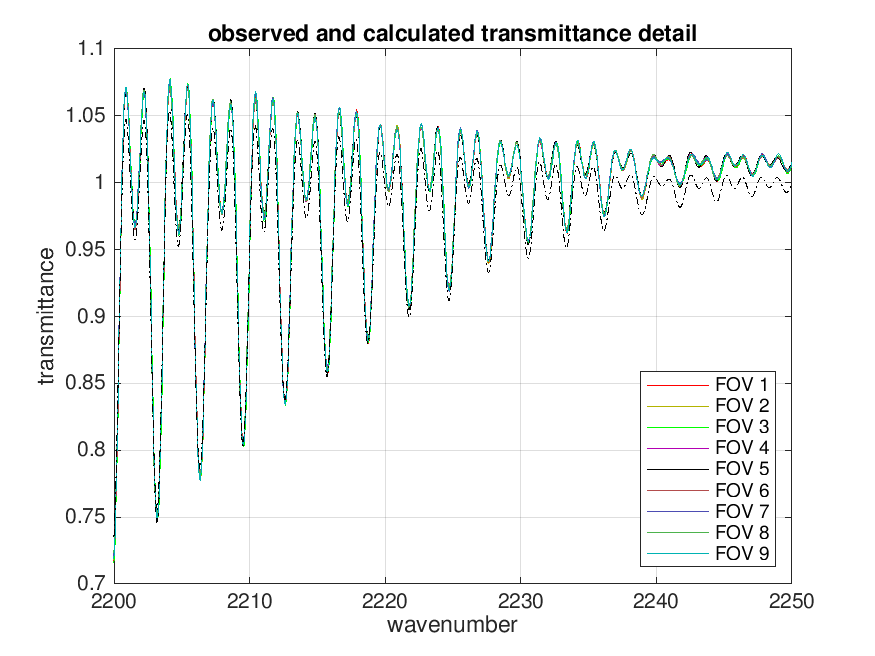
\includegraphics[width=\textwidth]{figures/spec_test2_CO_zoom.png}
  \end{centering}\vspace{3mm}

A detail from the previous plot. \\ The FOV to FOV consistency is
relatively good.  Note that we are using an older 41 torr calc here,
so some differences are to be expected.

\end{column}
\end{columns}
\end{frame}
%----------- slide --------------------------------------------------%
\begin{frame}
\frametitle{CO fitting overview}
\begin{columns}[t]
\begin{column}{0.5\textwidth}  
  \begin{centering}
  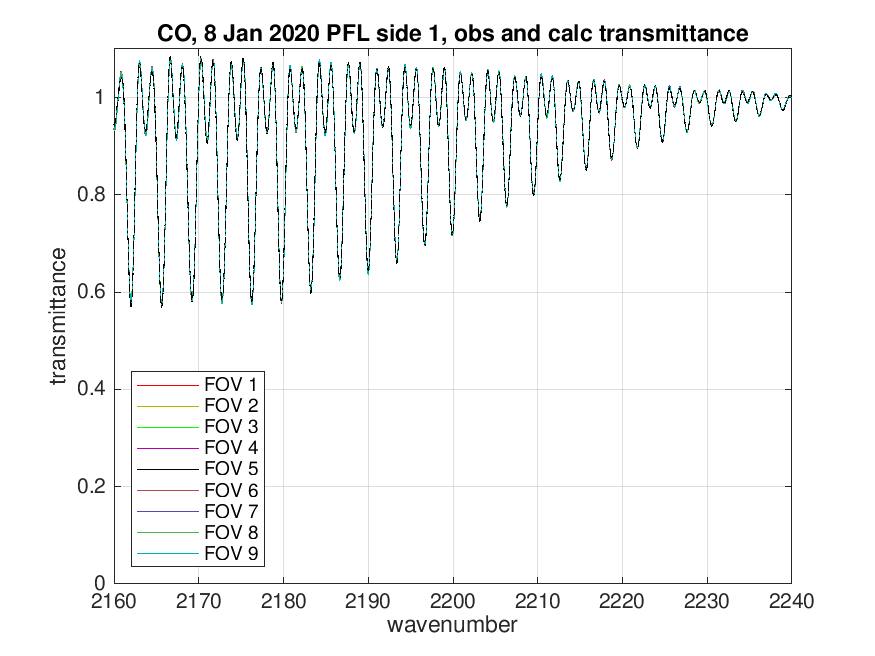
\includegraphics[width=\textwidth]{figures/CO_obs_and_calc.png}
  \end{centering}\vspace{3mm}

Observed and calculated transmittance for all FOVs, over the fitting
interval.  At this level of detail we see all values are very close.

\end{column}

\begin{column}{0.5\textwidth}
  \begin{centering}
  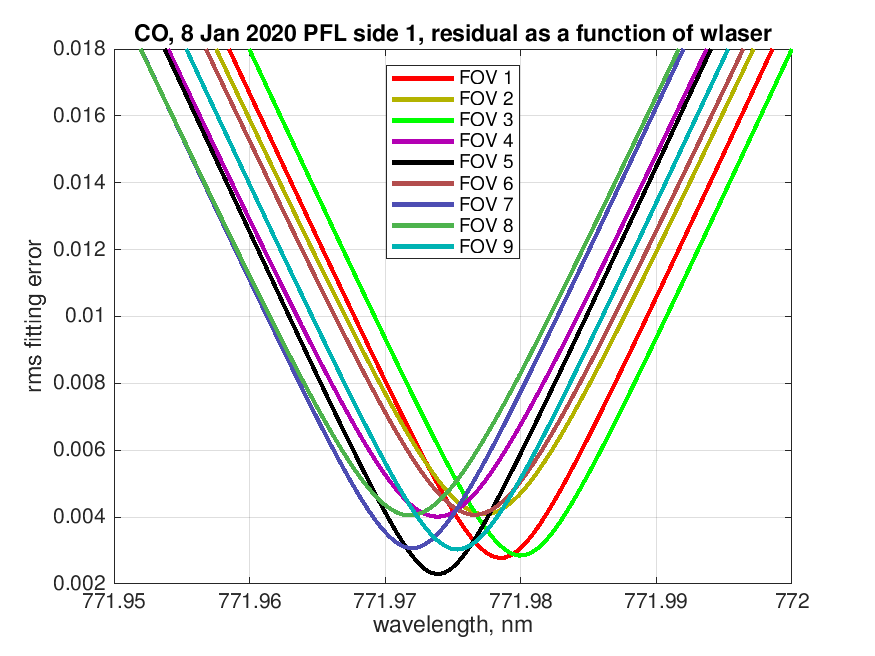
\includegraphics[width=\textwidth]{figures/CO_wlaser_fit.png}
  \end{centering}\vspace{3mm}

Residuals $\rms(a\cdot\tauobs + b - \taucal)$ over the fitting
interval as a function of metrology laser wavelength, for each FOV.

\end{column}
\end{columns}
\end{frame}
%----------- slide --------------------------------------------------%
\begin{frame}
\frametitle{CO obs minus calc breakouts}
\begin{columns}[t]
\begin{column}{0.5\textwidth}
  \begin{centering}
  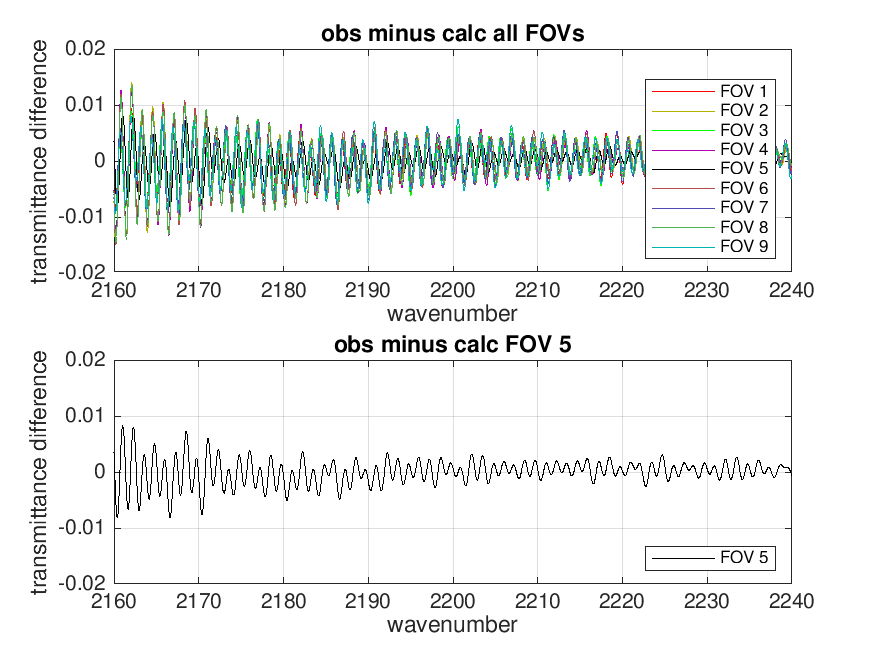
\includegraphics[width=\textwidth]{figures/CO_breakout_1.png}
  \end{centering}\vspace{3mm}

Observed minus calculated transmittance for all FOVs and for FOV~5
alone, over the fitting interval.

\end{column}
\begin{column}{0.5\textwidth}  
  \begin{centering}
  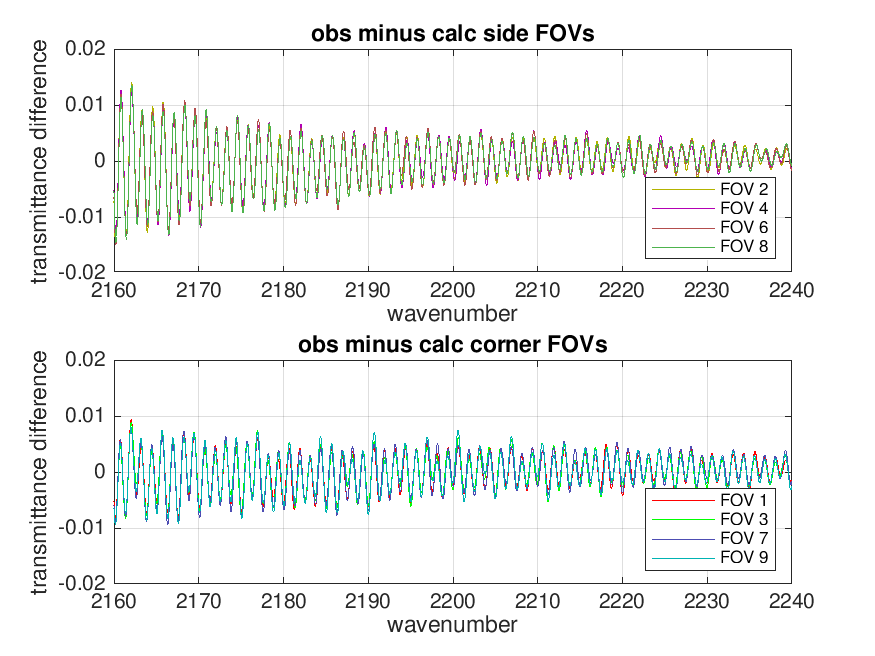
\includegraphics[width=\textwidth]{figures/CO_breakout_2.png}
  \end{centering}\vspace{3mm}

Observed minus calculated transmittance for side and corner FOVs,
over the fitting interval.

\end{column}
\end{columns}
\end{frame}
%----------- slide --------------------------------------------------%
\begin{frame}[fragile]
\frametitle{CO tabulated residuals}

  metrology laser absolute residuals, ppm
\begin{semiverbatim}\scriptsize
      1.94     4.53    10.36         7   4   1
      1.94     4.53     9.07         8   5   2
      6.48     8.42    12.31         9   6   3
\end{semiverbatim}

  metrology laser relative residuals, ppm
\begin{semiverbatim}\scriptsize
     -2.59     0.00     5.83         7   4   1
     -2.59     0.00     4.53         8   5   2
      1.94     3.89     7.77         9   6   3
\end{semiverbatim}

     regression fitting weights and residuals
\begin{semiverbatim}\scriptsize
 FOV   "a"       "b"     dmin     wmin      wfov
  1   0.938    0.0469   0.0028    10.36   771.9784 
  2   0.943    0.0429   0.0041     9.07   771.9774 
  3   0.940    0.0456   0.0028    12.31   771.9799 
  4   0.946    0.0387   0.0040     4.53   771.9739 
  5   0.940    0.0447   0.0023     4.53   771.9739 
  6   0.945    0.0399   0.0041     8.42   771.9769 
  7   0.945    0.0402   0.0031     1.94   771.9719 
  8   0.948    0.0372   0.0041     1.94   771.9719 
  9   0.939    0.0459   0.0030     6.48   771.9754 
\end{semiverbatim}

\end{frame}
%----------- slide --------------------------------------------------%
\begin{frame}[label={sec:orgdc40122}]{Focal Plane Fits to CH\textsubscript{4} PPM Shifts}
\begin{small}

\begin{itemize}
\item Neon already increased from Engr. Pkt by 16.7 ppm

\item Metrology laser offsets from gas cell spectra (ppm)
\end{itemize}
\begin{center}
\begin{tabular}{rrr}
-0.65 & 2.59 & 7.77\\
0.65 & 5.18 & 8.42\\
5.18 & 9.07 & 13.60\\
\end{tabular}
\end{center}

\begin{itemize}
\item Optimum focal plane offsets, radial magnification
\end{itemize}
\begin{center}
\begin{tabular}{rrl}
dx & dy & rdr\\
-158 & +214 & \textasciitilde{}32\\
\hline
unc   dx & unc   dy & unc rdr\\
38 & 38 & \textasciitilde{}25\\
\end{tabular}
\end{center}

\begin{itemize}
\item Metrology laser residuals from (relative) ppm fit
\end{itemize}
\begin{center}
\begin{tabular}{rrr}
-0.24 & 0.08 & -0.49\\
0.95 & 0 & 1.37\\
-0.05 & -0.37 & -0.23\\
\end{tabular}
\end{center}
\end{small}
\end{frame}

\begin{frame}[label={sec:org7d3bfb9}]{Focal Plane Fits to CO\textsubscript{2} PPM Shifts}
\begin{small}

\begin{itemize}
\item Metrology laser offsets from gas cell spectra (ppm)
\end{itemize}
\begin{center}
\begin{tabular}{rrr}
-3.24 & 1.94 & 7.12\\
-3.24 & 5.18 & 9.07\\
1.30 & 7.12 & 11.01\\
\end{tabular}
\end{center}

\begin{itemize}
\item Optimum focal plane offsets, radial magnification
\end{itemize}
\begin{center}
\begin{tabular}{rrl}
dx & dy & rdr\\
-118 & +280 & \textasciitilde{}44\\
\hline
unc   dx & unc   dy & unc rdr\\
58 & 58 & \textasciitilde{}44\\
\end{tabular}
\end{center}

\begin{itemize}
\item Metrology laser residuals from (relative) ppm fit
\end{itemize}
\begin{center}
\begin{tabular}{rrr}
-0.72 & 0.21 & -0.31\\
2.30 & 0 & 0.76\\
-0.75 & -0.44 & 0.37\\
\end{tabular}
\end{center}
\end{small}
\end{frame}


\begin{frame}[label={sec:org7fd0465}]{Focal Plane Fits to CO PPM Shifts}
\begin{small}

\begin{itemize}
\item Metrology laser offsets from gas cell spectra (ppm)
\end{itemize}
\begin{center}
\begin{tabular}{rrr}
1.94 & 4.53 & 10.36\\
1.94 & 4.53 & 9.07\\
6.48 & 8.42 & 12.31\\
\end{tabular}
\end{center}

\begin{itemize}
\item Optimum focal plane offsets, radial magnification
\end{itemize}
\begin{center}
\begin{tabular}{rrl}
dx & dy & rdr\\
-90 & +186 & \textasciitilde{}103\\
\hline
unc   dx & unc   dy & unc rdr\\
36 & 36 & \textasciitilde{}24\\
\end{tabular}
\end{center}

\begin{itemize}
\item Metrology laser residuals from (relative) ppm fit
\end{itemize}
\begin{center}
\begin{tabular}{rrr}
0.49 & -0.15 & -0.82\\
0.62 & 0 & 0.60\\
-0.61 & -0.59 & 0.71\\
\end{tabular}
\end{center}
\end{small}
\end{frame}
%----------- slide --------------------------------------------------%
\begin{frame}
\frametitle{Conclusions}
\begin{itemize}

  \item We have done a preliminary analysis of the PFL Plateau 20
    CH$_4$, CO$_2$, and CO gas cell tests, and compared these with
    calculated reference truth.  Initial results are promising, but
    could be improved with better test interval subsetting and
    transmittance calcs.

  \item It's not clear how much of this analysis can be automated.
    At a minimum it seems like a good idea to browse the data stream
    over time, as we have been doing, before chosing test subsets.

  \item These tests should probably be run at whatever operational
    resolution is chosen.  We do not truncate the interferograms for
    any resolution mode, as discussed in past presentations, and
    there are small differences.

\end{itemize}
\end{frame}
%----------- slide --------------------------------------------------%

\end{document}

